\appendix \subsection{Summary of the Multinomial Logistic Regression Model} \label{appendix:mlrm_formula}
Family: categorical \newline
Data: Training dataset (Number of observations: 19973 days of 67 brood cycles) \newline
Draws: 4 chains, each with iter = 2000; warmup = 1000; thin = 1; total post-warmup draws = 4000 \newline
Formula:
\begin{align*}
BroodPhase = Sex + 95MCP^2 + MeanNestDistance + ResidenceTime + Revisitations \\
+ Sex x (95MCP^2 + MeanNestDistance + ResidenceTime + Revisitations) \\
+ ResidenceTime x Revisitations + nDailyLocations + (1 | YearID)
\end{align*}

\vspace{1\baselineskip}

\noindent Group-Level Effects: YearID (Number of levels: 155)

\begin{table}[H]
\footnotesize{
\begin{center}
\begin{tabular}{| p{5.3cm} | p{1.1cm} | p{1.1cm} | p{0.85cm} | p{0.95cm} | p{0.5cm} | p{1.3cm} | p{1.2cm} |} 
\hline
& \textbf{Estimate} & \textbf{Est.Error} & \textbf{l-95\%} & \textbf{u-95\%} & \textbf{Rhat} & \textbf{Bulk\_ESS} & \textbf{Tail\_ESS} \\
\hline
sd(Incubating\_Intercept) & 1.02 & 0.07 & 0.89 & 1.17 & 1.01 & 980 & 1750 \\ 
\hline
sd(Feeding\_Intercept) & 1.00 & 0.07 & 0.88 & 1.14 & 1.00 & 905 & 1781 \\
\hline
\end{tabular}
\end{center}
}
\end{table}


\noindent Population-Level Effects:

\begin{table}[H]
\footnotesize{
\begin{center}
\begin{tabular}{| p{5.3cm} | p{1.1cm} | p{1.1cm} | p{0.85cm} | p{0.95cm} | p{0.5cm} | p{1.3cm} | p{1.2cm} |}
\hline
& \textbf{Estimate} & \textbf{Est.Error} & \textbf{l-95\%} & \textbf{u-95\%} & \textbf{Rhat} & \textbf{Bulk\_ESS} & \textbf{Tail\_ESS} \\
\hline
\footnotesize{Incubating\_Intercept} & -1.40 & 0.23 & -1.86 & -0.95 & 1.00 & 1147 & 1968 \\ 
\hline
\footnotesize{Incubating\_Sex(f)} & 0.06 & 0.27 & -0.47 & 0.62 & 1.00 & 892 & 1356 \\ 
\hline
\footnotesize{Incubating\_95MCP} & 1.64 & 0.25 & 1.14 & 2.13 & 1.00 & 2157 & 2724 \\ 
\hline
\footnotesize{Incubating\_MeanNestDistance} & -3.24 & 0.32 & -3.89 & -2.61 & 1.00 & 1711 & 2591 \\ 
\hline
\footnotesize{Incubating\_ResidenceTime} & -0.24 & 0.34 & -0.92 & 0.40 & 1.00 & 2898 & 2634 \\ 
\hline
\footnotesize{Incubating\_Revisitations} & 7.54 & 0.26 & 7.04 & 8.05 & 1.00 & 2492 & 3103 \\ 
\hline
\footnotesize{Incubating\_nDailyLocations} & -1.26 & 0.19 & -1.63 & -0.89 & 1.00 & 3922 & 3097 \\ 
\hline
\footnotesize{Incubating\_Sex(f):95MCP} & -20.47 & 1.98 & -24.50 & -16.69 & 1.00 & 3299 & 2699 \\ 
\hline
\footnotesize{Incubating\_Sex(f):MeanNestDistance} & -1.86 & 0.98 & -3.82 & -0.02 & 1.00 & 1923 & 2678 \\ 
\hline
\footnotesize{Incubating\_Sex(f):ResidenceTime} & 6.66 & 0.40 & 5.88 & 7.49 & 1.00 & 1922 & 2714 \\ 
\hline
\footnotesize{Incubating\_Sex(f):Revisitations} & -5.55 & 0.42 & -6.38 & -4.72 & 1.00 & 1739 & 2397 \\ 
\hline
\footnotesize{Incubating\_ResidenceTime:Revisitations} & -2.39 & 0.42 & -3.20 & -1.54 & 1.00 & 3026 & 2925 \\ 
\hline
\footnotesize{Feeding\_Intercept} & -3.21 & 0.22 & -3.63 & -2.77 & 1.01 & 617 & 1758 \\
\hline
\footnotesize{Feeding\_Sex(f)} & -0.71 & 0.24 & -1.18 & -0.24 & 1.00 & 489 & 1212 \\ 
\hline
\footnotesize{Feeding\_95MCP} & 3.07 & 0.18 & 2.73 & 3.42 & 1.00 & 2005 & 2376 \\ 
\hline
\footnotesize{Feeding\_MeanNestDistance} & -2.95 & 0.24 & -3.42 & -2.49 & 1.00 & 1618 & 2604 \\ 
\hline
\footnotesize{Feeding\_ResidenceTime} & 1.50 & 0.28 & 0.94 & 2.03 & 1.00 & 2716 & 2874 \\ 
\hline
\footnotesize{Feeding\_Revisitations} & 3.12 & 0.22 & 2.71 & 3.56 & 1.00 & 2258 & 3098 \\ 
\hline
\footnotesize{Feeding\_nDailyLocations} & 3.37 & 0.19 & 3.01 & 3.75 & 1.00 & 4274 & 3239 \\ 
\hline
\footnotesize{Feeding\_Sex(f):95MCP} & -3.52 & 0.45 & -4.42 & -2.67 & 1.00 & 1726 & 2649 \\ 
\hline
\footnotesize{Feeding\_Sex(f):MeanNestDistance} & -4.41 & 0.56 & -5.55 & -3.31 & 1.00 & 1313 & 2065 \\ 
\hline
\footnotesize{Feeding\_Sex(f):ResidenceTime} & 3.56 & 0.37 & 2.82 & 4.31 & 1.00 & 1991 & 2650 \\ 
\hline
\footnotesize{Feeding\_Sex(f):Revisitations} & 0.40 & 0.37 & -0.32 & 1.12 & 1.00 & 1743 & 2646 \\ 
\hline
\footnotesize{Feeding\_ResidenceTime:Revisitations} & -3.34 & 0.36 & -4.03 & -2.62 & 1.00 & 3117 & 3267 \\ 
\hline
\end{tabular}
\end{center}
}
\end{table}



\newpage
\subsection{Raw Model Predictions for the Test Dataset} \label{appendix:mlrm_predictions_test}
\begin{figure}[H]
\centering
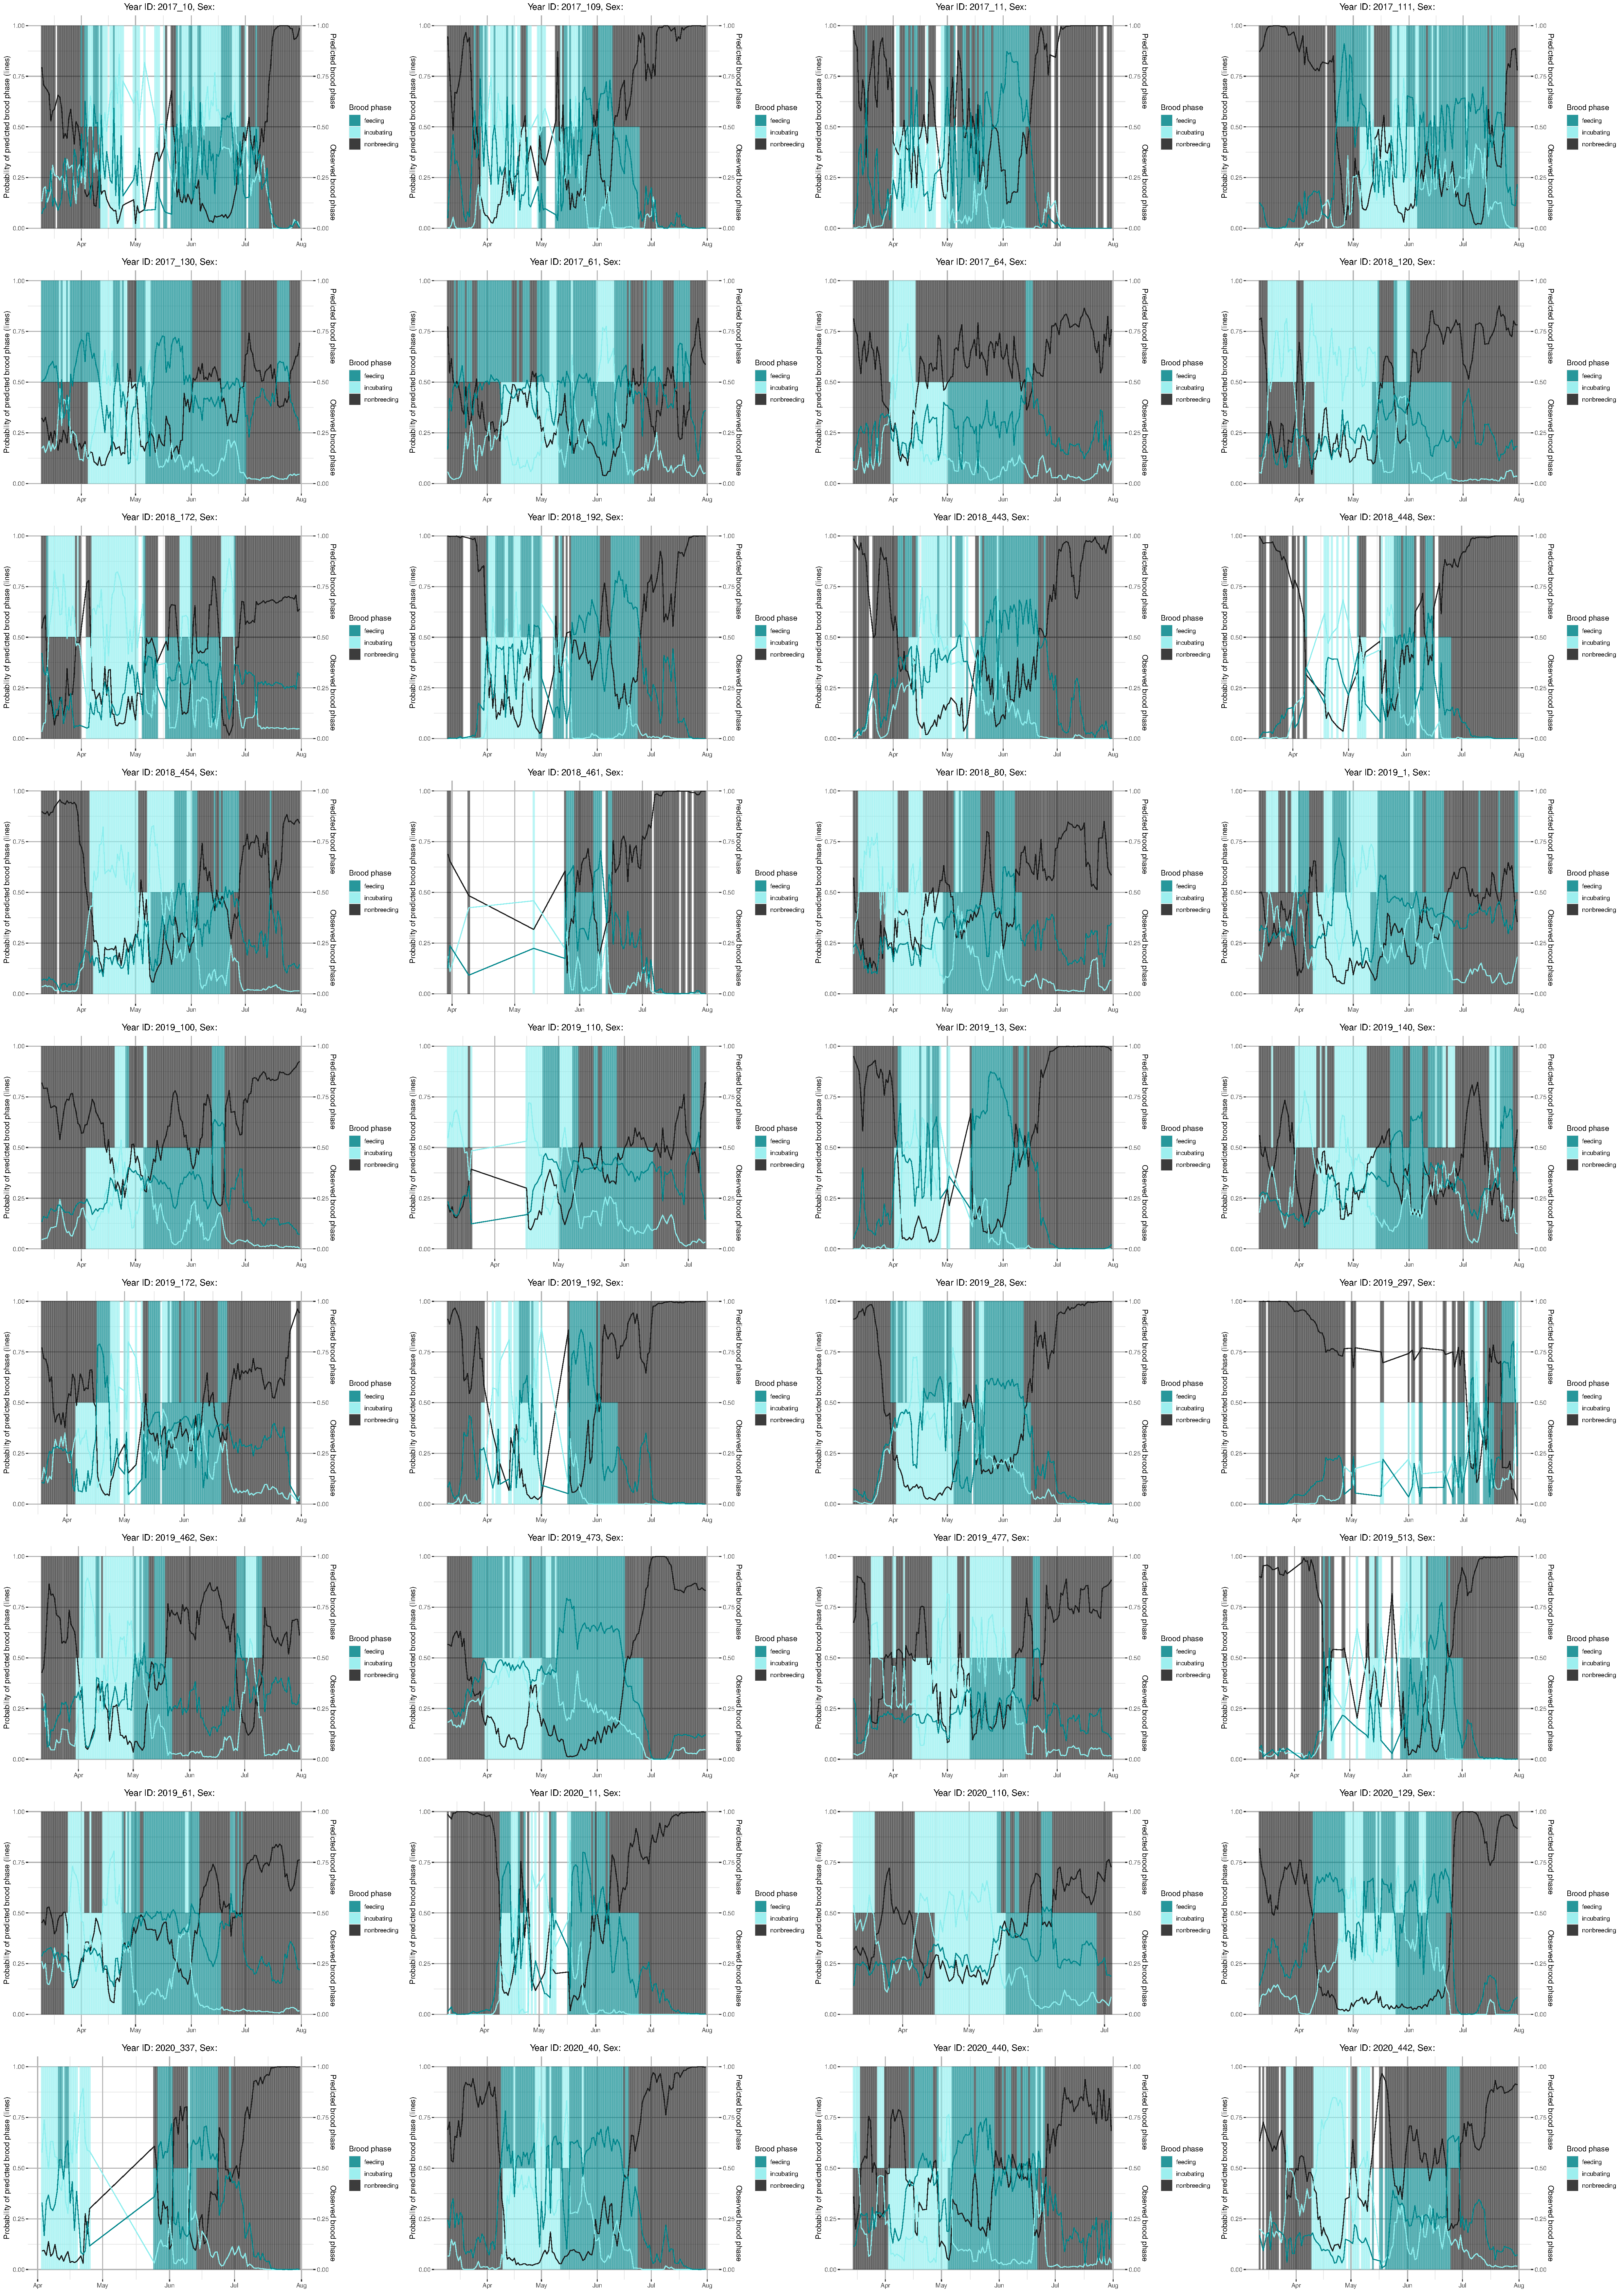
\includegraphics[width=1\textwidth]{figures/appendix/01_predictions_test_data_a.pdf}
\end{figure}
\newpage
\begin{figure}[H]
\centering
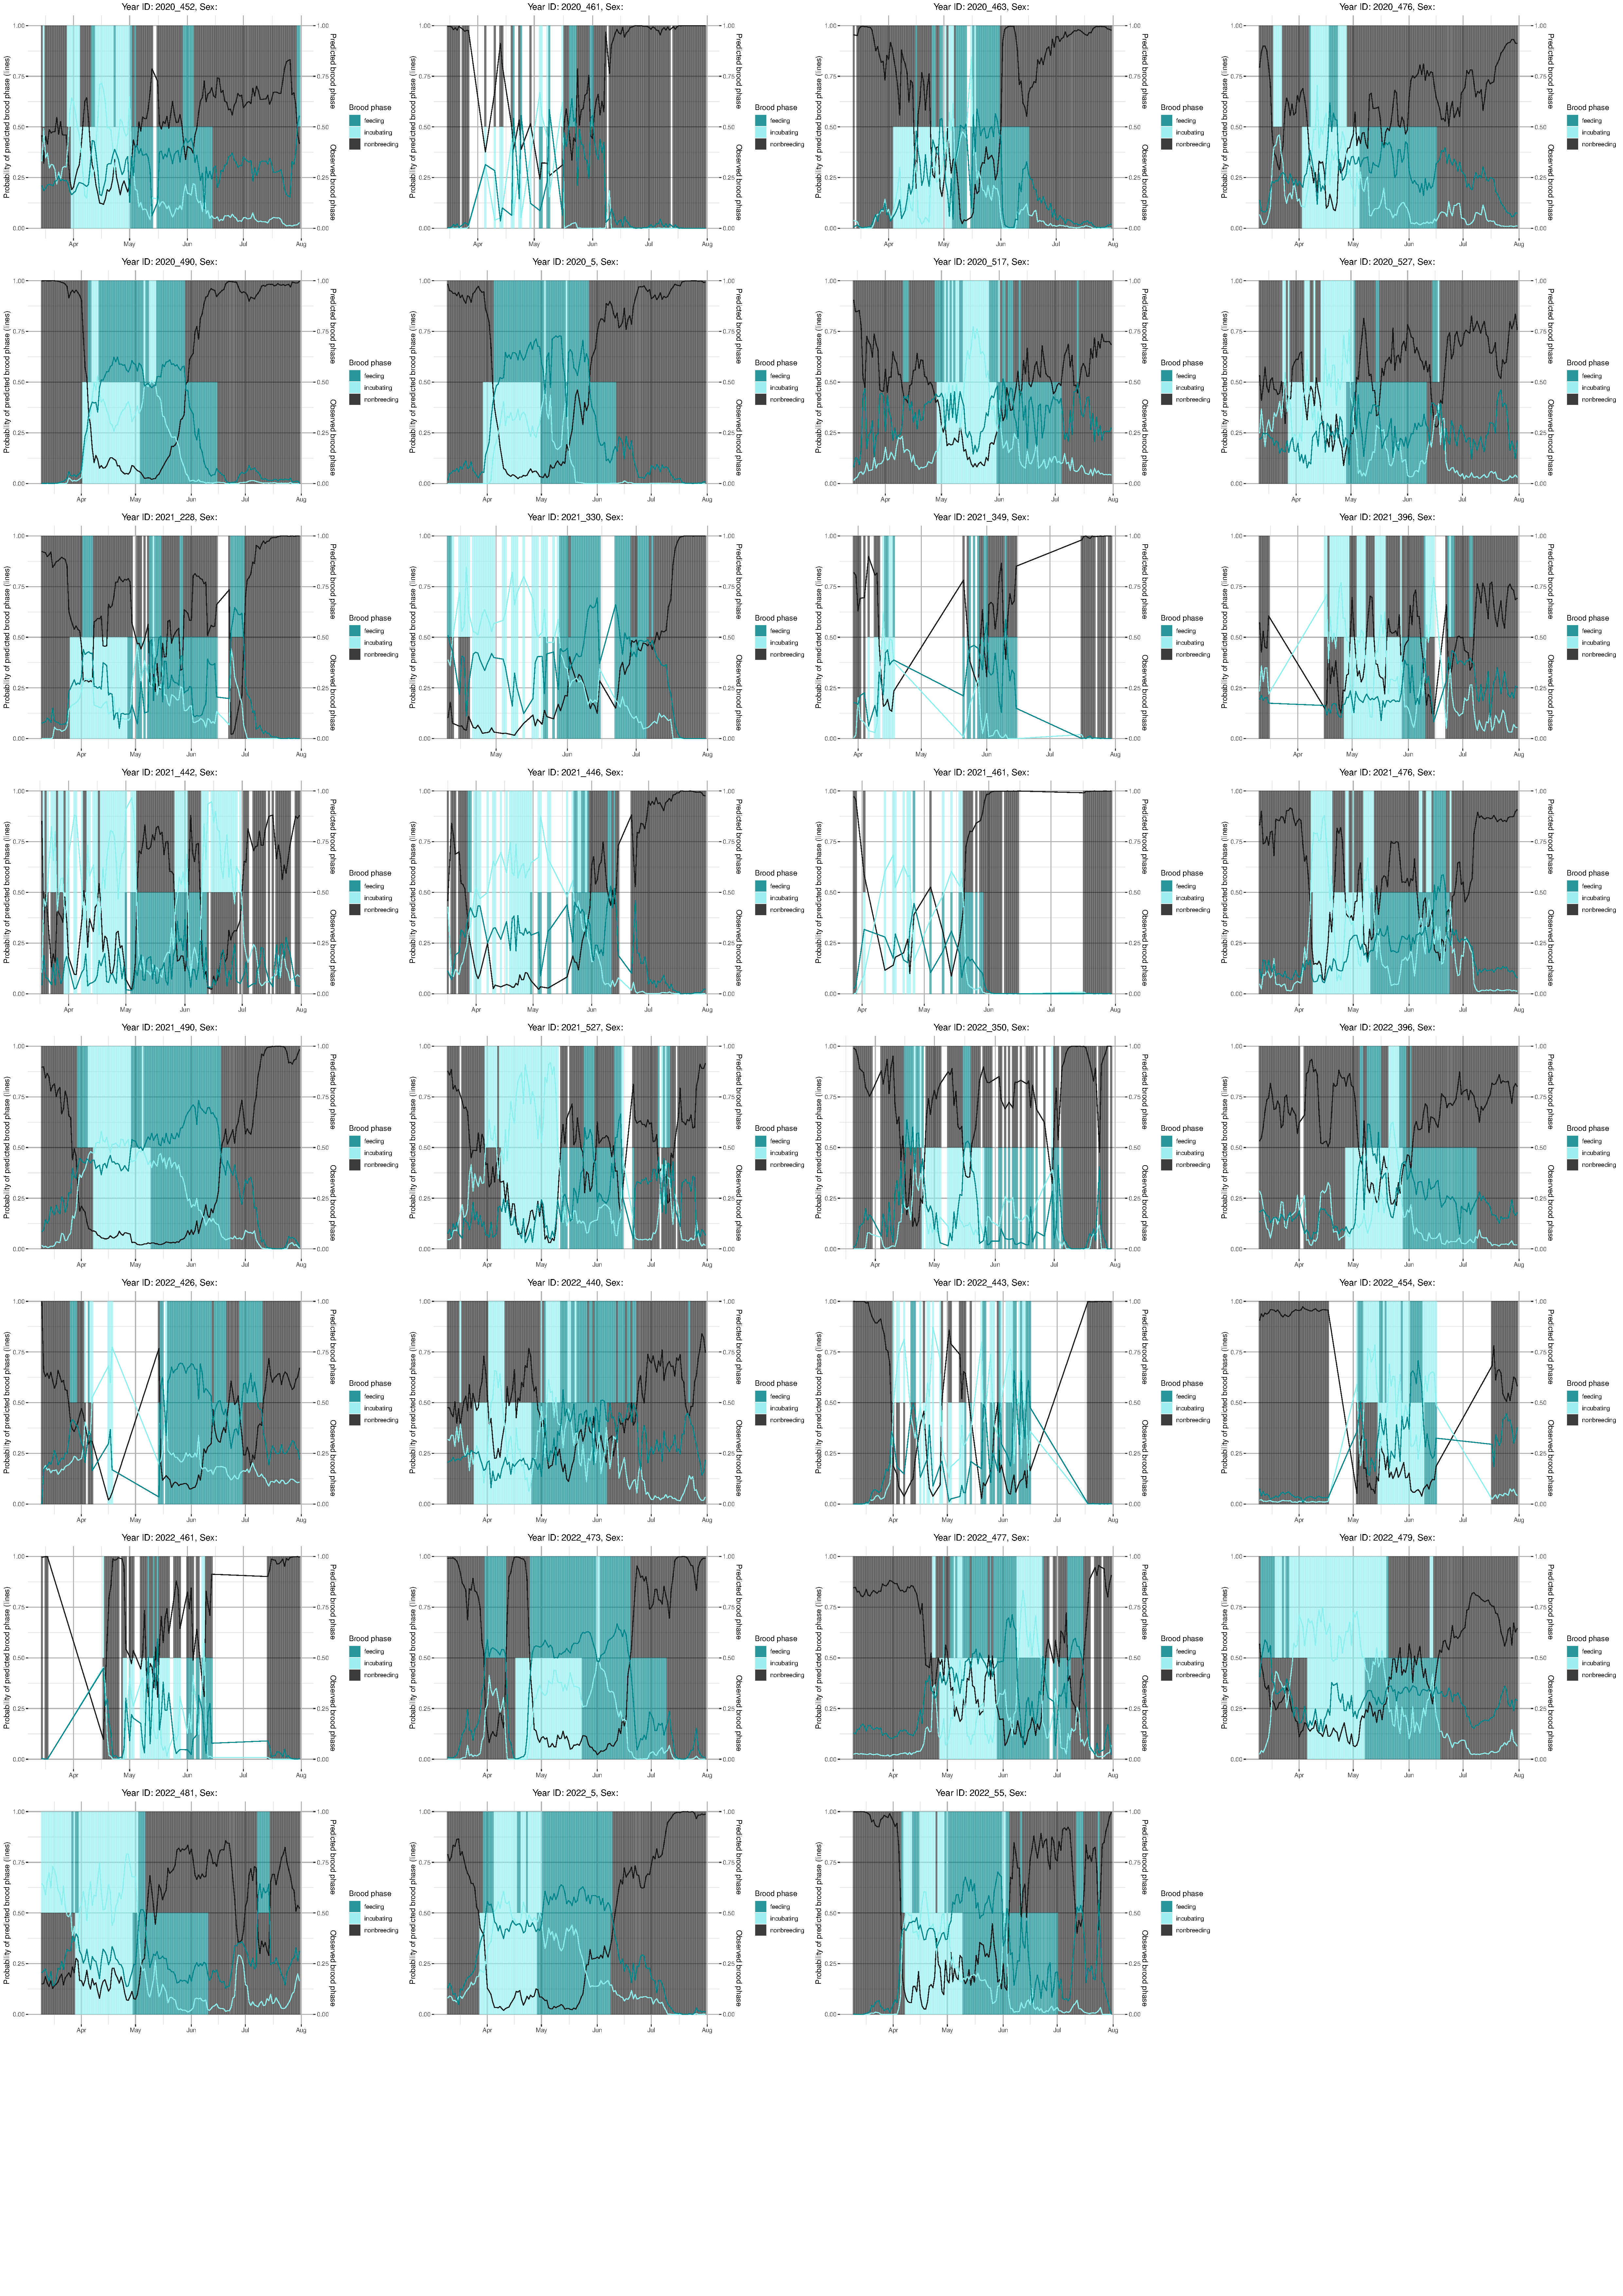
\includegraphics[width=1\textwidth]{figures/appendix/02_predictions_test_data_b.pdf}
\end{figure}



\newpage
\subsection{Raw Model Predictions for Non-Breeding Red Kites} \label{appendix:mlrm_predictions_nonbreeding}
\begin{figure}[H]
\centering
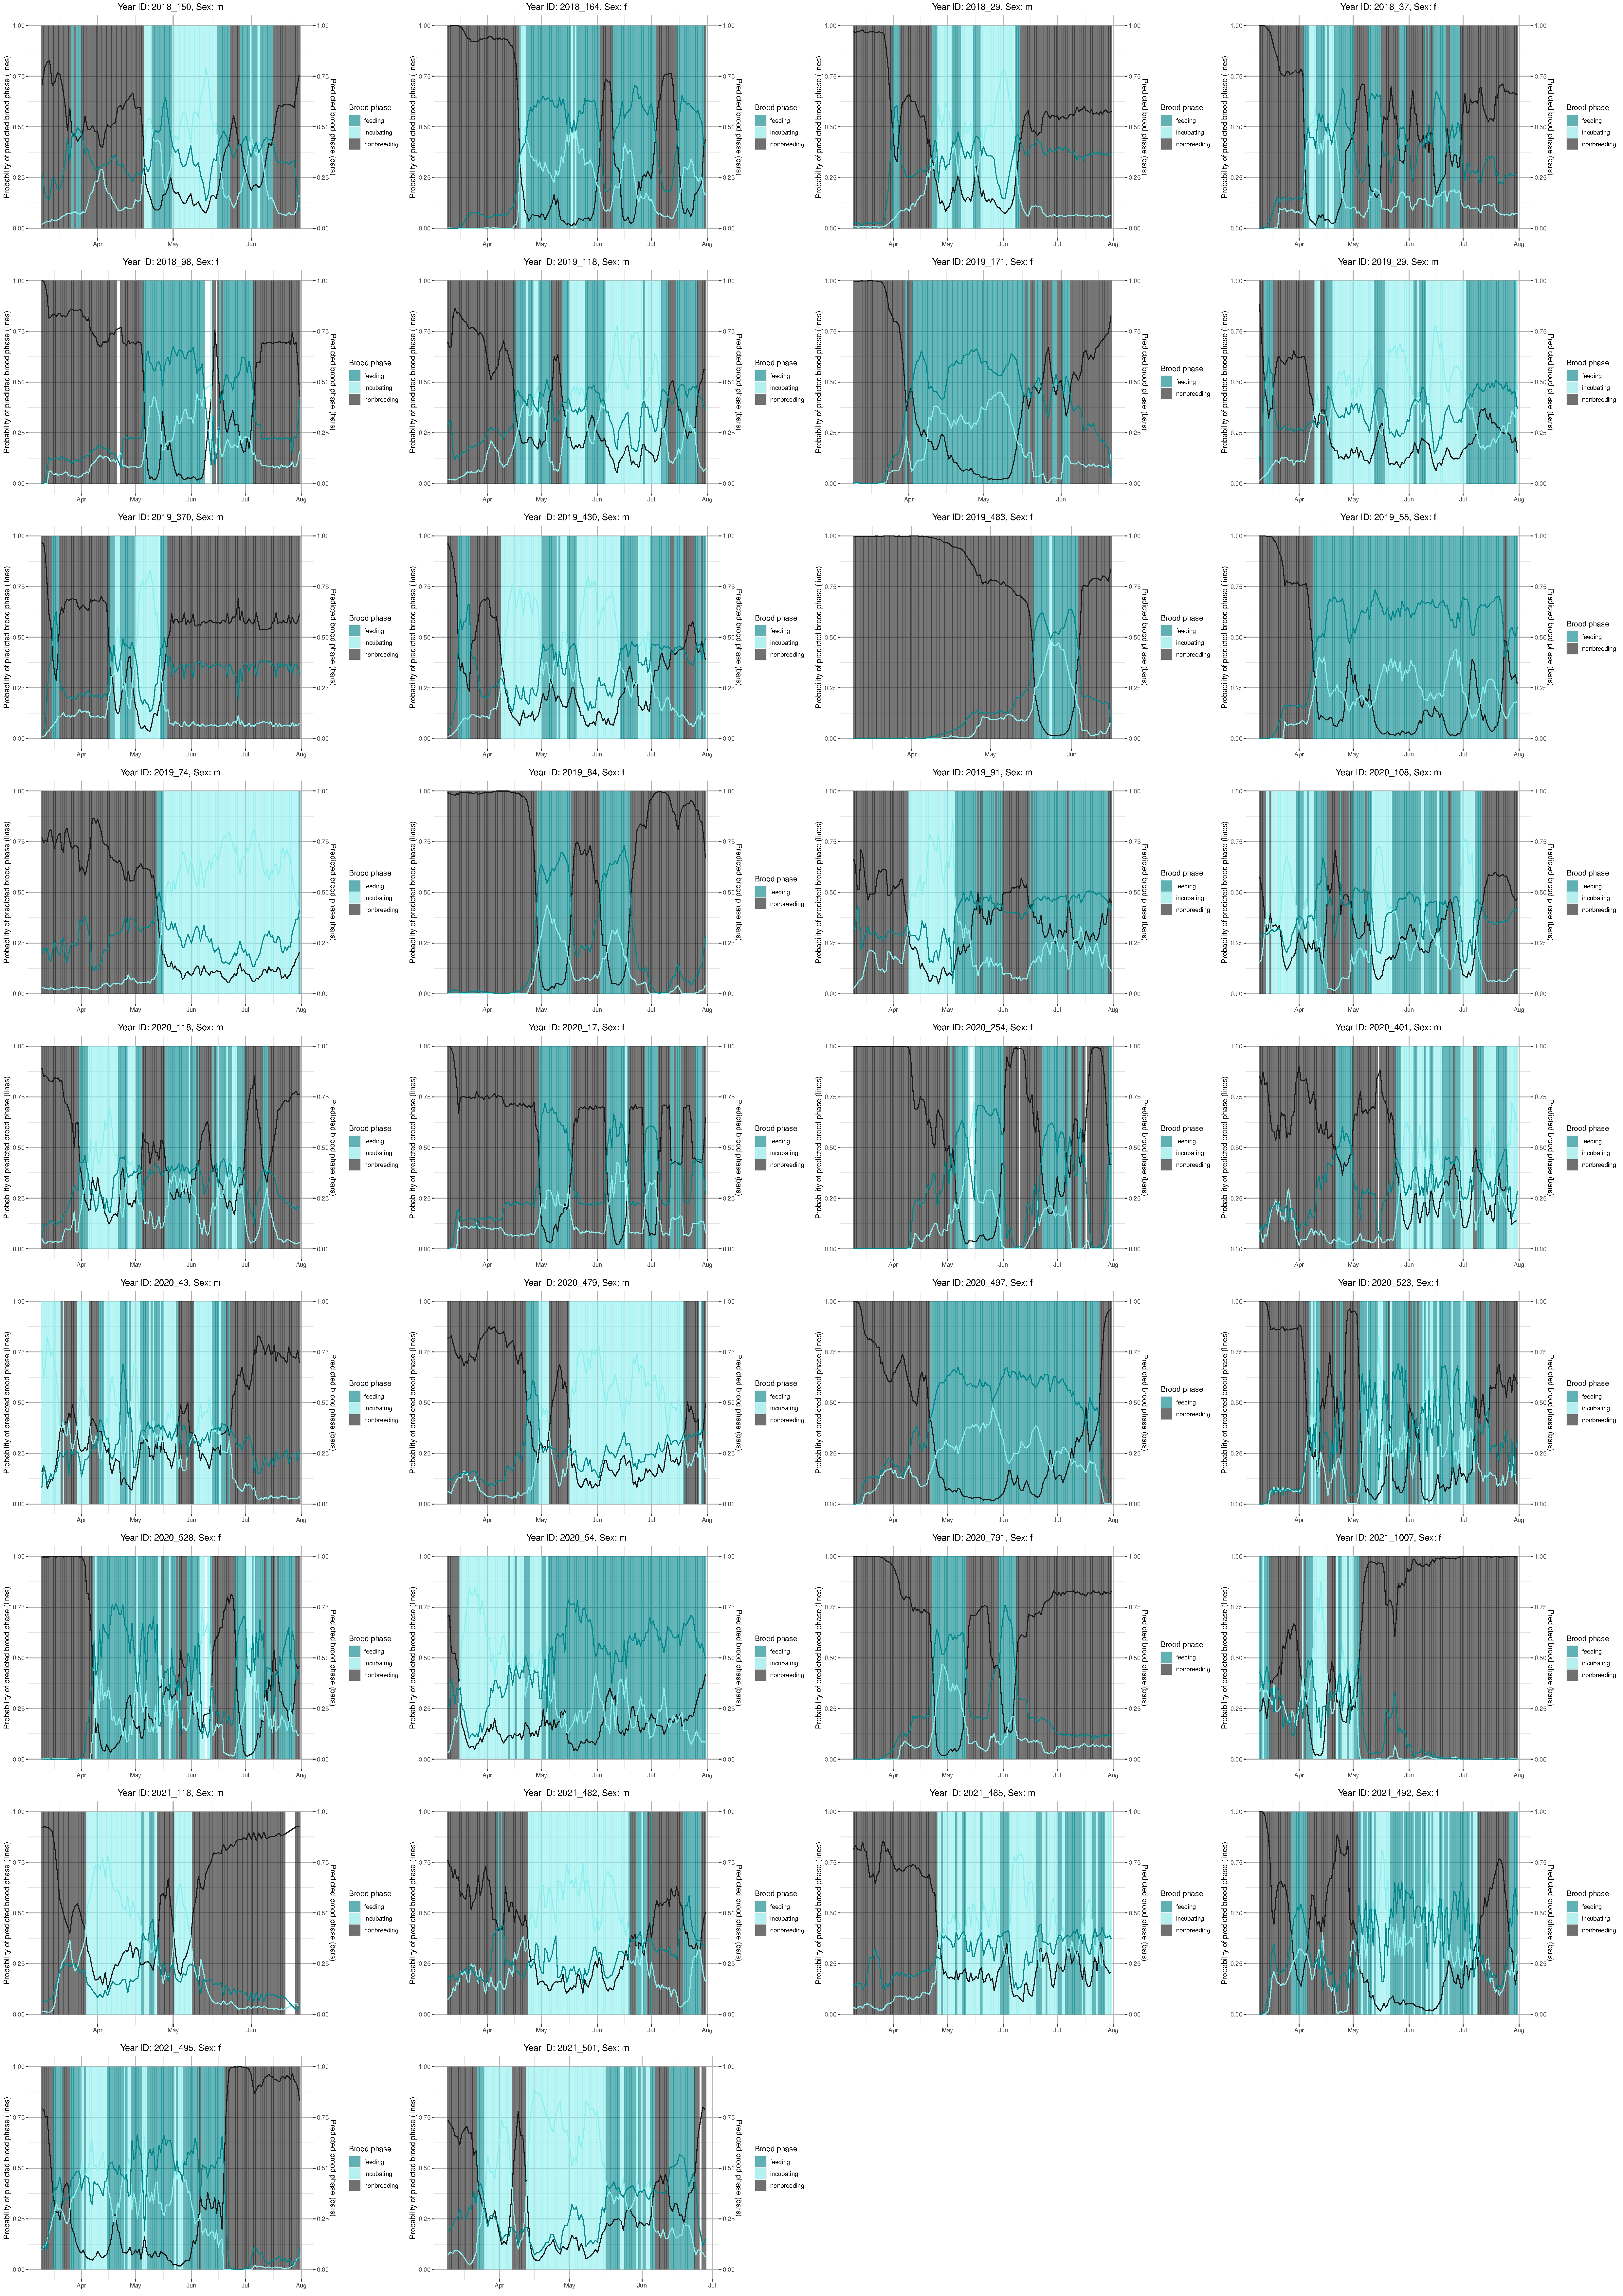
\includegraphics[width=1\textwidth]{figures/appendix/03_predictions_nonbreeders.pdf}
\end{figure}



\newpage
\subsection{Raw Model Predictions for Red Kites in Thuringia} \label{appendix:mlrm_predictions_thuringia}
\begin{figure}[H]
\centering
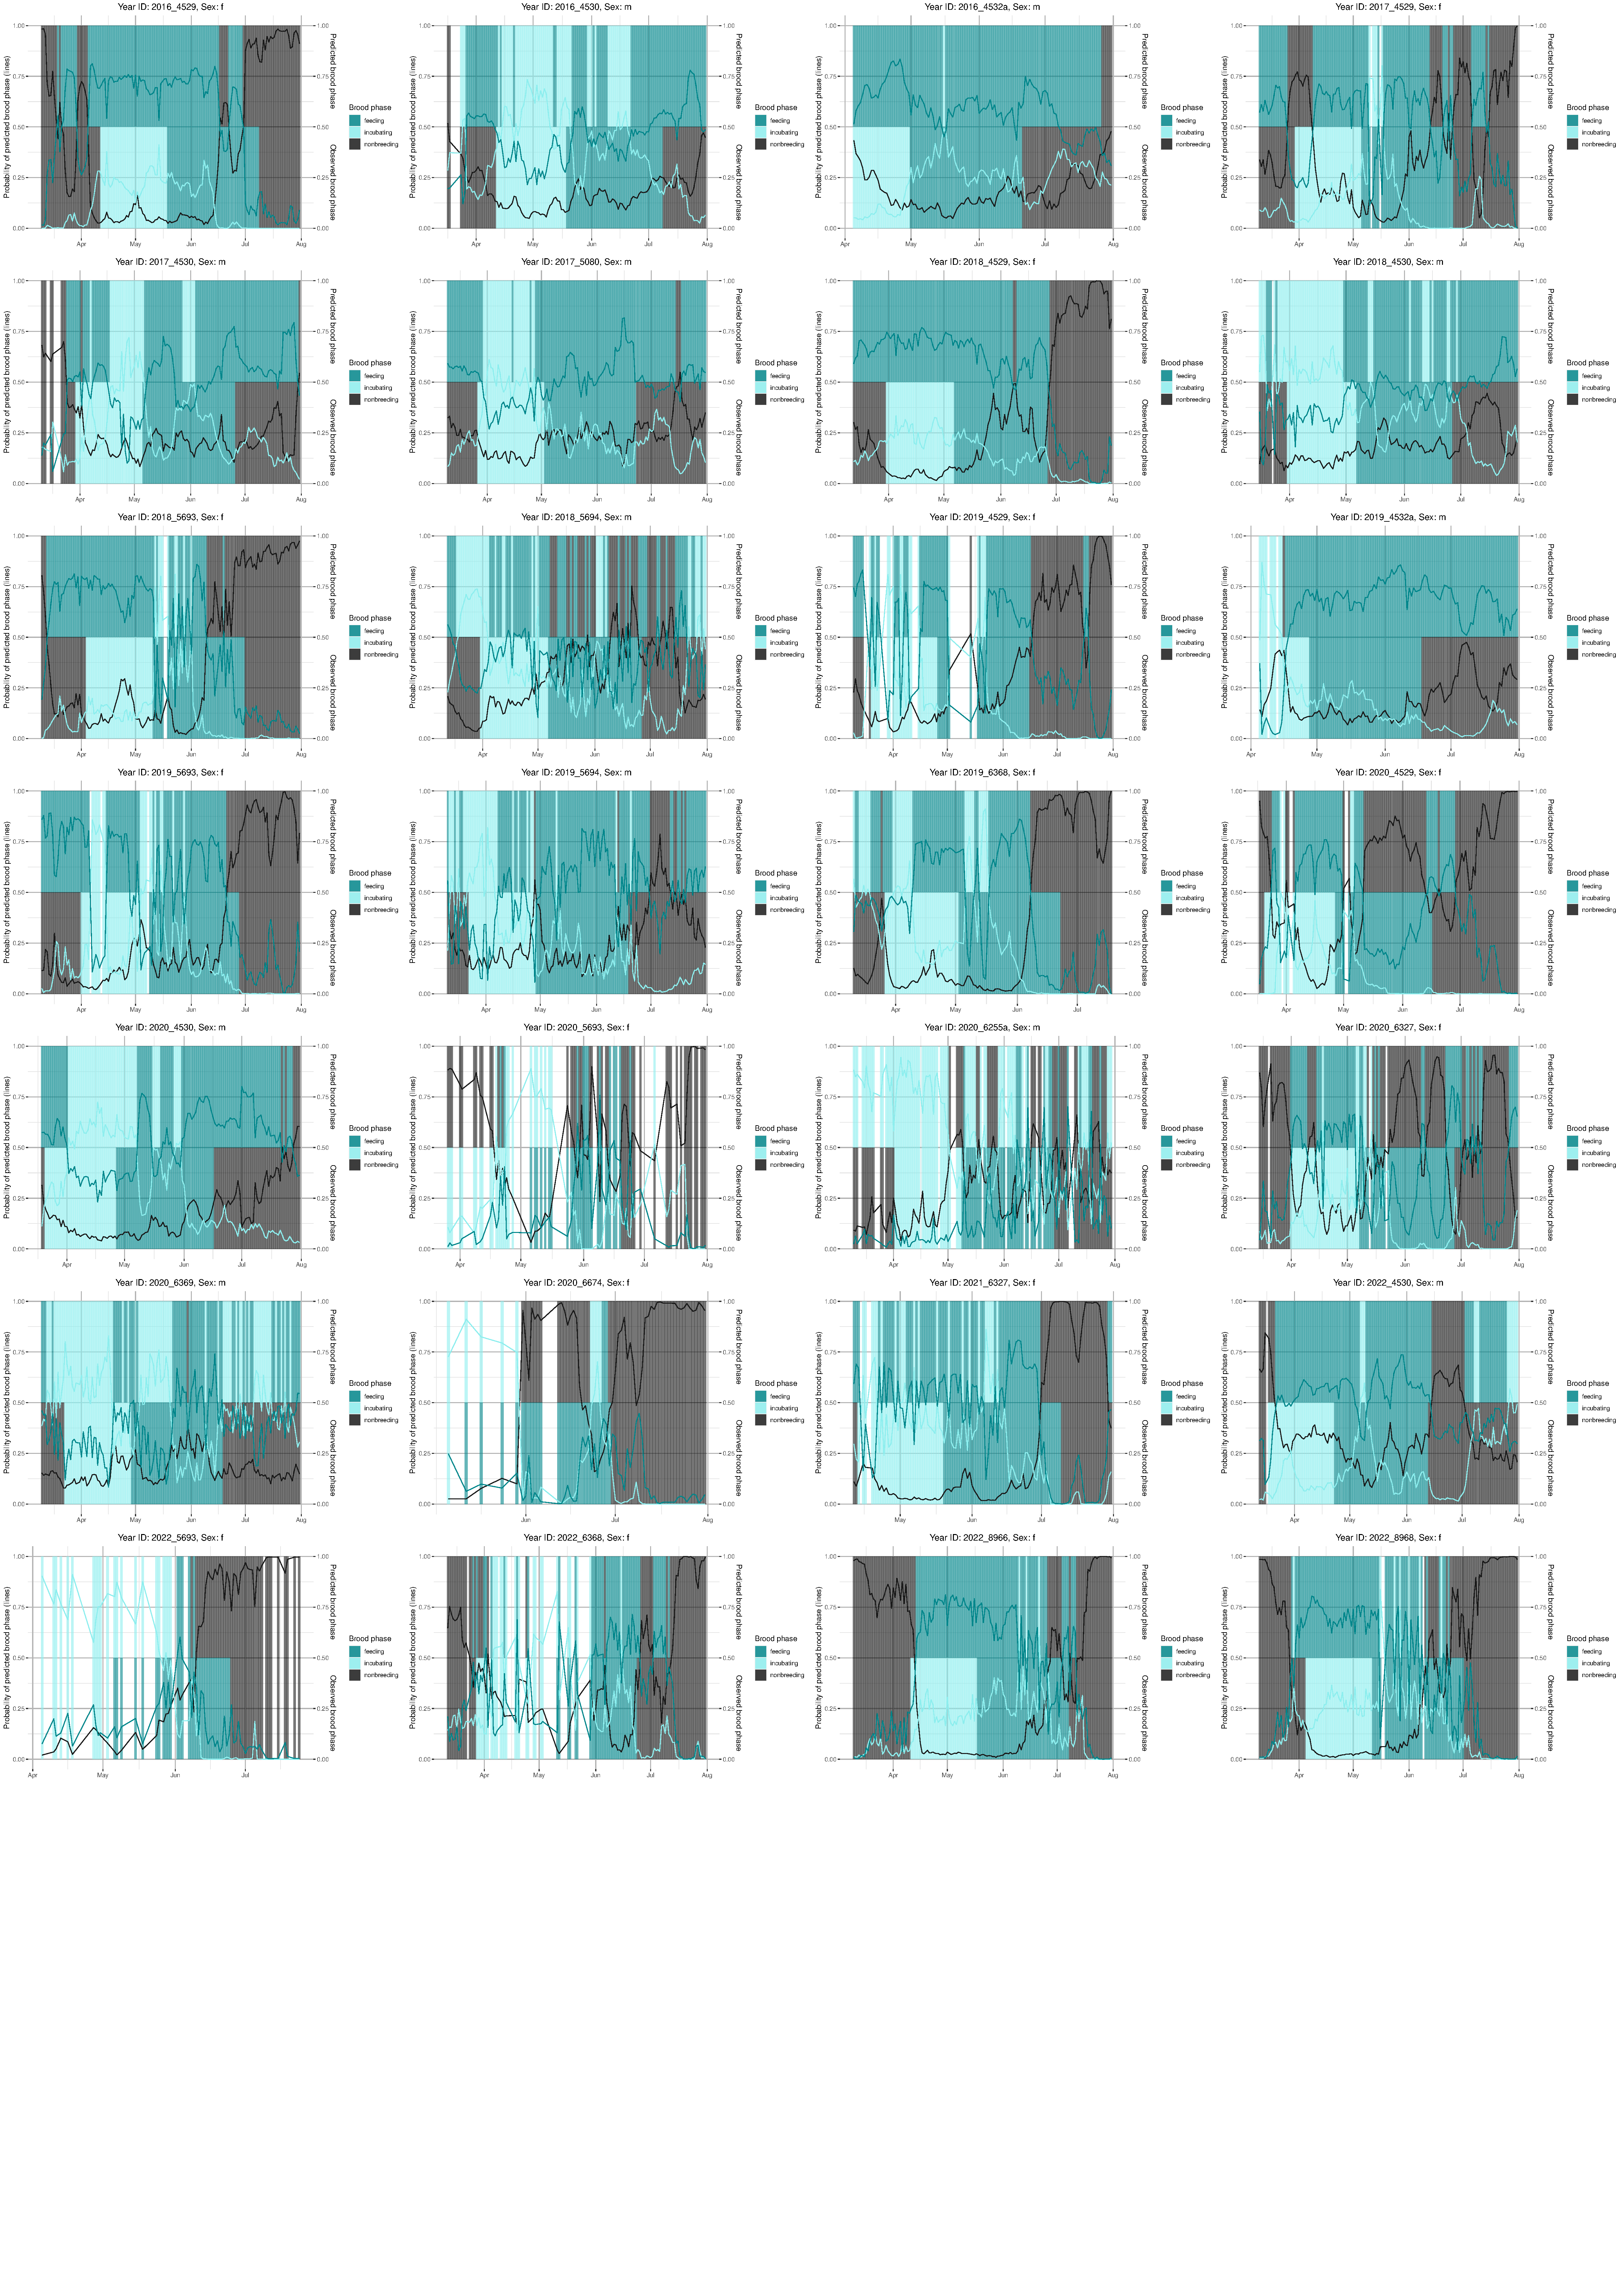
\includegraphics[width=1\textwidth]{figures/appendix/04_predictions_thuringia.pdf}
\end{figure}